
%% bare_conf.tex
%% V1.3
%% 2007/01/11
%% by Michael Shell
%% See:
%% http://www.michaelshell.org/
%% for current contact information.
%%
%% This is a skeleton file demonstrating the use of IEEEtran.cls
%% (requires IEEEtran.cls version 1.7 or later) with an IEEE conference paper.
%%
%% Support sites:
%% http://www.michaelshell.org/tex/ieeetran/
%% http://www.ctan.org/tex-archive/macros/latex/contrib/IEEEtran/
%% and
%% http://www.ieee.org/

%%*************************************************************************
%% Legal Notice:
%% This code is offered as-is without any warranty either expressed or
%% implied; without even the implied warranty of MERCHANTABILITY or
%% FITNESS FOR A PARTICULAR PURPOSE!
%% User assumes all risk.
%% In no event shall IEEE or any contributor to this code be liable for
%% any damages or losses, including, but not limited to, incidental,
%% consequential, or any other damages, resulting from the use or misuse
%% of any information contained here.
%%
%% All comments are the opinions of their respective authors and are not
%% necessarily endorsed by the IEEE.
%%
%% This work is distributed under the LaTeX Project Public License (LPPL)
%% ( http://www.latex-project.org/ ) version 1.3, and may be freely used,
%% distributed and modified. A copy of the LPPL, version 1.3, is included
%% in the base LaTeX documentation of all distributions of LaTeX released
%% 2003/12/01 or later.
%% Retain all contribution notices and credits.
%% ** Modified files should be clearly indicated as such, including  **
%% ** renaming them and changing author support contact information. **
%%
%% File list of work: IEEEtran.cls, IEEEtran_HOWTO.pdf, bare_adv.tex,
%%                    bare_conf.tex, bare_jrnl.tex, bare_jrnl_compsoc.tex
%%*************************************************************************

% *** Authors should verify (and, if needed, correct) their LaTeX system  ***
% *** with the testflow diagnostic prior to trusting their LaTeX platform ***
% *** with production work. IEEE's font choices can trigger bugs that do  ***
% *** not appear when using other class files.                            ***
% The testflow support page is at:
% http://www.michaelshell.org/tex/testflow/



% Note that the a4paper option is mainly intended so that authors in
% countries using A4 can easily print to A4 and see how their papers will
% look in print - the typesetting of the document will not typically be
% affected with changes in paper size (but the bottom and side margins will).
% Use the testflow package mentioned above to verify correct handling of
% both paper sizes by the user's LaTeX system.
%
% Also note that the "draftcls" or "draftclsnofoot", not "draft", option
% should be used if it is desired that the figures are to be displayed in
% draft mode.
%
\documentclass[conference]{IEEEtran}
\usepackage{balance}  % to better equalize the last page
\usepackage{graphics} % for EPS, load graphicx instead
\usepackage{times}    % comment if you want LaTeX's default font
\usepackage{url}      % llt: nicely formatted URLs
\usepackage{multirow}
\usepackage{euscript}
\usepackage{url}
\usepackage{pstricks, pst-node}
\usepackage{textcomp}
\usepackage{stmaryrd}
\usepackage{epsfig}
\usepackage{subfigure}
\usepackage{booktabs}
\usepackage{graphicx}
\usepackage{float}
\usepackage{tabularx}
\usepackage{epstopdf}


\usepackage{graphicx}
\usepackage{latexsym}
\usepackage[fleqn]{amsmath}
\usepackage[varg]{txfonts}
\usepackage{float}

\usepackage{graphicx, graphics}
\usepackage{algorithmic}
\usepackage{tabularx}
\renewcommand{\algorithmicrequire}{\textbf{Input:}}
\renewcommand{\algorithmicensure}{\textbf{Output:}}

% Add the compsoc option for Computer Society conferences.
%
% If IEEEtran.cls has not been installed into the LaTeX system files,
% manually specify the path to it like:
% \documentclass[conference]{../sty/IEEEtran}


\makeatletter
\newenvironment{tablehere}
  {\def\@captype{table}}
  {}

\newenvironment{figurehere}
  {\def\@captype{figure}}
  {}
\makeatother




% Some very useful LaTeX packages include:
% (uncomment the ones you want to load)


% *** MISC UTILITY PACKAGES ***
%
%\usepackage{ifpdf}
% Heiko Oberdiek's ifpdf.sty is very useful if you need conditional
% compilation based on whether the output is pdf or dvi.
% usage:
% \ifpdf
%   % pdf code
% \else
%   % dvi code
% \fi
% The latest version of ifpdf.sty can be obtained from:
% http://www.ctan.org/tex-archive/macros/latex/contrib/oberdiek/
% Also, note that IEEEtran.cls V1.7 and later provides a builtin
% \ifCLASSINFOpdf conditional that works the same way.
% When switching from latex to pdflatex and vice-versa, the compiler may
% have to be run twice to clear warning/error messages.






% *** CITATION PACKAGES ***
%
%\usepackage{cite}
% cite.sty was written by Donald Arseneau
% V1.6 and later of IEEEtran pre-defines the format of the cite.sty package
% \cite{} output to follow that of IEEE. Loading the cite package will
% result in citation numbers being automatically sorted and properly
% "compressed/ranged". e.g., [1], [9], [2], [7], [5], [6] without using
% cite.sty will become [1], [2], [5]--[7], [9] using cite.sty. cite.sty's
% \cite will automatically add leading space, if needed. Use cite.sty's
% noadjust option (cite.sty V3.8 and later) if you want to turn this off.
% cite.sty is already installed on most LaTeX systems. Be sure and use
% version 4.0 (2003-05-27) and later if using hyperref.sty. cite.sty does
% not currently provide for hyperlinked citations.
% The latest version can be obtained at:
% http://www.ctan.org/tex-archive/macros/latex/contrib/cite/
% The documentation is contained in the cite.sty file itself.






% *** GRAPHICS RELATED PACKAGES ***
%
\ifCLASSINFOpdf
  % \usepackage[pdftex]{graphicx}
  % declare the path(s) where your graphic files are
  % \graphicspath{{../pdf/}{../jpeg/}}
  % and their extensions so you won't have to specify these with
  % every instance of \includegraphics
  % \DeclareGraphicsExtensions{.pdf,.jpeg,.png}
\else
  % or other class option (dvipsone, dvipdf, if not using dvips). graphicx
  % will default to the driver specified in the system graphics.cfg if no
  % driver is specified.
  % \usepackage[dvips]{graphicx}
  % declare the path(s) where your graphic files are
  % \graphicspath{{../eps/}}
  % and their extensions so you won't have to specify these with
  % every instance of \includegraphics
  % \DeclareGraphicsExtensions{.eps}
\fi
% graphicx was written by David Carlisle and Sebastian Rahtz. It is
% required if you want graphics, photos, etc. graphicx.sty is already
% installed on most LaTeX systems. The latest version and documentation can
% be obtained at:
% http://www.ctan.org/tex-archive/macros/latex/required/graphics/
% Another good source of documentation is "Using Imported Graphics in
% LaTeX2e" by Keith Reckdahl which can be found as epslatex.ps or
% epslatex.pdf at: http://www.ctan.org/tex-archive/info/
%
% latex, and pdflatex in dvi mode, support graphics in encapsulated
% postscript (.eps) format. pdflatex in pdf mode supports graphics
% in .pdf, .jpeg, .png and .mps (metapost) formats. Users should ensure
% that all non-photo figures use a vector format (.eps, .pdf, .mps) and
% not a bitmapped formats (.jpeg, .png). IEEE frowns on bitmapped formats
% which can result in "jaggedy"/blurry rendering of lines and letters as
% well as large increases in file sizes.
%
% You can find documentation about the pdfTeX application at:
% http://www.tug.org/applications/pdftex





% *** MATH PACKAGES ***
%
%\usepackage[cmex10]{amsmath}
% A popular package from the American Mathematical Society that provides
% many useful and powerful commands for dealing with mathematics. If using
% it, be sure to load this package with the cmex10 option to ensure that
% only type 1 fonts will utilized at all point sizes. Without this option,
% it is possible that some math symbols, particularly those within
% footnotes, will be rendered in bitmap form which will result in a
% document that can not be IEEE Xplore compliant!
%
% Also, note that the amsmath package sets \interdisplaylinepenalty to 10000
% thus preventing page breaks from occurring within multiline equations. Use:
%\interdisplaylinepenalty=2500
% after loading amsmath to restore such page breaks as IEEEtran.cls normally
% does. amsmath.sty is already installed on most LaTeX systems. The latest
% version and documentation can be obtained at:
% http://www.ctan.org/tex-archive/macros/latex/required/amslatex/math/





% *** SPECIALIZED LIST PACKAGES ***
%
%\usepackage{algorithmic}
% algorithmic.sty was written by Peter Williams and Rogerio Brito.
% This package provides an algorithmic environment fo describing algorithms.
% You can use the algorithmic environment in-text or within a figure
% environment to provide for a floating algorithm. Do NOT use the algorithm
% floating environment provided by algorithm.sty (by the same authors) or
% algorithm2e.sty (by Christophe Fiorio) as IEEE does not use dedicated
% algorithm float types and packages that provide these will not provide
% correct IEEE style captions. The latest version and documentation of
% algorithmic.sty can be obtained at:
% http://www.ctan.org/tex-archive/macros/latex/contrib/algorithms/
% There is also a support site at:
% http://algorithms.berlios.de/index.html
% Also of interest may be the (relatively newer and more customizable)
% algorithmicx.sty package by Szasz Janos:
% http://www.ctan.org/tex-archive/macros/latex/contrib/algorithmicx/




% *** ALIGNMENT PACKAGES ***
%
%\usepackage{array}
% Frank Mittelbach's and David Carlisle's array.sty patches and improves
% the standard LaTeX2e array and tabular environments to provide better
% appearance and additional user controls. As the default LaTeX2e table
% generation code is lacking to the point of almost being broken with
% respect to the quality of the end results, all users are strongly
% advised to use an enhanced (at the very least that provided by array.sty)
% set of table tools. array.sty is already installed on most systems. The
% latest version and documentation can be obtained at:
% http://www.ctan.org/tex-archive/macros/latex/required/tools/


%\usepackage{mdwmath}
%\usepackage{mdwtab}
% Also highly recommended is Mark Wooding's extremely powerful MDW tools,
% especially mdwmath.sty and mdwtab.sty which are used to format equations
% and tables, respectively. The MDWtools set is already installed on most
% LaTeX systems. The lastest version and documentation is available at:
% http://www.ctan.org/tex-archive/macros/latex/contrib/mdwtools/


% IEEEtran contains the IEEEeqnarray family of commands that can be used to
% generate multiline equations as well as matrices, tables, etc., of high
% quality.


%\usepackage{eqparbox}
% Also of notable interest is Scott Pakin's eqparbox package for creating
% (automatically sized) equal width boxes - aka "natural width parboxes".
% Available at:
% http://www.ctan.org/tex-archive/macros/latex/contrib/eqparbox/





% *** SUBFIGURE PACKAGES ***
%\usepackage[tight,footnotesize]{subfigure}
% subfigure.sty was written by Steven Douglas Cochran. This package makes it
% easy to put subfigures in your figures. e.g., "Figure 1a and 1b". For IEEE
% work, it is a good idea to load it with the tight package option to reduce
% the amount of white space around the subfigures. subfigure.sty is already
% installed on most LaTeX systems. The latest version and documentation can
% be obtained at:
% http://www.ctan.org/tex-archive/obsolete/macros/latex/contrib/subfigure/
% subfigure.sty has been superceeded by subfig.sty.



%\usepackage[caption=false]{caption}
%\usepackage[font=footnotesize]{subfig}
% subfig.sty, also written by Steven Douglas Cochran, is the modern
% replacement for subfigure.sty. However, subfig.sty requires and
% automatically loads Axel Sommerfeldt's caption.sty which will override
% IEEEtran.cls handling of captions and this will result in nonIEEE style
% figure/table captions. To prevent this problem, be sure and preload
% caption.sty with its "caption=false" package option. This is will preserve
% IEEEtran.cls handing of captions. Version 1.3 (2005/06/28) and later
% (recommended due to many improvements over 1.2) of subfig.sty supports
% the caption=false option directly:
%\usepackage[caption=false,font=footnotesize]{subfig}
%
% The latest version and documentation can be obtained at:
% http://www.ctan.org/tex-archive/macros/latex/contrib/subfig/
% The latest version and documentation of caption.sty can be obtained at:
% http://www.ctan.org/tex-archive/macros/latex/contrib/caption/




% *** FLOAT PACKAGES ***
%
%\usepackage{fixltx2e}
% fixltx2e, the successor to the earlier fix2col.sty, was written by
% Frank Mittelbach and David Carlisle. This package corrects a few problems
% in the LaTeX2e kernel, the most notable of which is that in current
% LaTeX2e releases, the ordering of single and double column floats is not
% guaranteed to be preserved. Thus, an unpatched LaTeX2e can allow a
% single column figure to be placed prior to an earlier double column
% figure. The latest version and documentation can be found at:
% http://www.ctan.org/tex-archive/macros/latex/base/



%\usepackage{stfloats}
% stfloats.sty was written by Sigitas Tolusis. This package gives LaTeX2e
% the ability to do double column floats at the bottom of the page as well
% as the top. (e.g., "\begin{figure*}[!b]" is not normally possible in
% LaTeX2e). It also provides a command:
%\fnbelowfloat
% to enable the placement of footnotes below bottom floats (the standard
% LaTeX2e kernel puts them above bottom floats). This is an invasive package
% which rewrites many portions of the LaTeX2e float routines. It may not work
% with other packages that modify the LaTeX2e float routines. The latest
% version and documentation can be obtained at:
% http://www.ctan.org/tex-archive/macros/latex/contrib/sttools/
% Documentation is contained in the stfloats.sty comments as well as in the
% presfull.pdf file. Do not use the stfloats baselinefloat ability as IEEE
% does not allow \baselineskip to stretch. Authors submitting work to the
% IEEE should note that IEEE rarely uses double column equations and
% that authors should try to avoid such use. Do not be tempted to use the
% cuted.sty or midfloat.sty packages (also by Sigitas Tolusis) as IEEE does
% not format its papers in such ways.





% *** PDF, URL AND HYPERLINK PACKAGES ***
%
%\usepackage{url}
% url.sty was written by Donald Arseneau. It provides better support for
% handling and breaking URLs. url.sty is already installed on most LaTeX
% systems. The latest version can be obtained at:
% http://www.ctan.org/tex-archive/macros/latex/contrib/misc/
% Read the url.sty source comments for usage information. Basically,
% \url{my_url_here}.





% *** Do not adjust lengths that control margins, column widths, etc. ***
% *** Do not use packages that alter fonts (such as pslatex).         ***
% There should be no need to do such things with IEEEtran.cls V1.6 and later.
% (Unless specifically asked to do so by the journal or conference you plan
% to submit to, of course. )


% correct bad hyphenation here
\hyphenation{op-tical net-works semi-conduc-tor}


\begin{document}
\title{Automatic Evaluation of Generative Dialogue Systems: An Empirical Study}

\author{
%\IEEEauthorblockN{Wenge Rong}
%\IEEEauthorblockA{Research Institute of Beihang in Shenzhen\\
%VU Park, High-tech Industrial Estate\\
%Shenzhen 518000, China\\
%w.rong@buaa.edu.cn}
%\and
\IEEEauthorblockN{Cong Feng, Wenge Rong, Jianxin Yang, Yuanxin Ouyang, Zhang Xiong}
\IEEEauthorblockA{School of Computer Science and Engineering, Beihang University, Beijing 100191, China\\
\{congfeng, w.rong, yjx17, oyyx, xiongz\}@buaa.edu.cn}
}

\maketitle

\begin{abstract}
	Evaluating generative dialogue systems with automatic metrics is a difficult problem. It has been shown that the word-overlap metrics such as BLEU and the word-embedding metrics correlate poorly with human judgments. In this paper, we highlight yet another problem of evaluation with metrics through an empirical study. We show that regardless of the correlation with human judgments, the scores of these metrics do not correlate well with one another, which means fine-tuning the system on one set of metrics may yield a gotcha when testing with another set of metrics. This infeasibility again adds to the ineffectiveness of evaluation done alone with metrics. To the end of utilizing metrics at its best, we offer several pragmatic suggestions on the use of automatic metrics to avoid the issue of metric inconsistency.
\end{abstract}

\begin{IEEEkeywords}
Automatic Metrics, Dialogue Response Generation, Chatbot
\end{IEEEkeywords}

\section{Introduction}

    The chat-oriented dialogue systems have seen a boom in the recent literature of dialogue systems. These systems are trained to make an appropriate response given a conversational context and can be applied to various chatbot applications, language education tools, and intelligent personal assistants. This setting is different from that of the traditional task-oriented dialogue systems, which are programmed to assist their users to complete a certain task, such as restaurant reservation and airline information acquisition. As a result, the chat-oriented dialogue systems cannot be evaluated in the same supervised setting as their task-oriented counterpart, which turns out to bring a new challenge.

    As an advanced approach to the chat-oriented system, the generative models based on neural networks feature end-to-end training with minimal hard-coded features and the ability to output fluent human-like sentences. Given a large corpus of context-response pairs, these neural models can learn language patterns and extract common-sense knowledge from the corpus in an unsupervised manner, making it a highly plausible solution to the response generation problem.

    The research community has made steady progress with the generative models. Vinyals et al. \cite{GoogleChatbot} applied the Seq2Seq model \cite{Seq2Seq} to generate responses to both technical queries in an IT helpdesk and open-ended questions such as \textit{what's the purpose of life?} Their model consistently outperformed a rule-based chatbot. However, generative models are not without problems. They incline to give meaningless responses to the questions they are incapable to handle, such as \textit{I don't know what you're talking about} and like any chat-oriented systems, their evaluation remains an open problem.

    Previous works of generative dialogue systems started by borrowing automatic metrics from the machine translation community, such as the popular BLEU \cite{BLEU} and METEOR \cite{METEOR}. However, the correlations between these borrowed metrics and human judgments were unclear and researchers generally fell back to human evaluation for better accuracy and reliability \cite{Shang,DCGM,VHRED}. Liu et al. performed an empirical study on how well these metrics correlated with human judgments \cite{HowNot}. They concluded that the metrics only correlated weakly with human judgments on the non-technical Twitter corpus and not at all on the technical Ubuntu Dialogue Corpus \cite{ubuntu_corpus}. They urged against the use of these metrics and called for the development of new automatic metrics that are more relevant to human judgments.

    In this paper, we followed the work of Liu et al.'s and investigated the behaviors of automatic metrics without human judgments. We analyzed both system-level and example-level scores to find out possible correlations. In particular, we drew samples from the example-level scores of different metrics and analyze the pairwise correlation of these samples. We found that some pairs of samples have a high correlation, while other pairs show a much lower one.

    Following these observations, we clustered the metrics based on the pairwise correlations of their corresponding samples. The results show that similar metrics tend to cluster together, indicating a high pairwise correlation within the same group. According to the experiment results, we argue that the scores given by dissimilar metrics have the risk of high inconsistency, which is yet another pitfall of using automatic metrics. Therefore, it is strongly recommended to choose consistent metrics for the ease of comparison across different settings.

\section{Related Work}
The most traditional way for paraphrase identification was based on simple lexical matching and vector-based similarity approach. The feasibility of exploiting string-based features on both word and character level has been revealed to some extent \cite{selfdef:conf/altw/WanDDP06}. In order to measure the similarity of texts, Mihalcea et al. used corpus-based and knowledge-based measures of similarity acquired from the word-level similarity \cite{DBLP:conf/aaai/MihalceaCS06}. Though this kind of approaches is easy to implement by statistical analysis in large text collections, the importances from semantic similarity's perspective is also widely mentioned, e.g., based on corpus like Wikipedia \cite{DBLP:conf/ijcai/GabrilovichM07}. Recently many work also utilised distributed representations like word embedding to calculate the word and/or sentence similarity \cite{DBLP:conf/icml/SantosZ14}. Besides the similarity realisation from word level, several works also proposed syntactic oriented solutions trying to integrate some external information into the paraphrase identification process. e.g., parse tree \cite{DBLP:conf/acl/DasS09}.

Besides the advanced feature engineering, a lot of machine learning based models are also proposed to solve this problem, e.g., SVM, KNN and etc \cite{DBLP:conf/fintal/KozarevaM06}. Recently, with the development of neural network, it is becoming interesting to ask if it will be helpful when advanced neural models integrated with sophisticated feature? In fact, many recent work has focused more on modelling with distributed representations and neural network architectures and one of the examples is CNN, which has been applied into many natural language processing tasks. For instance, CNN is used for relation extraction and relation classification tasks \cite{nguyen2015relation}. CNNs are also used for learning sentence-level representation with semantically meaning \cite{DBLP:conf/cikm/ShenHGDM14}. Kim proposed a CNN architecture on various classification datasets, including Sentiment Analysis and Topic Categorization tasks \cite{DBLP:conf/emnlp/Kim14}. This CNN architecture is powerful and achieves good result though very simply. It uses the concatenated word embeddings as input, containing the semantic information of words. Kalchbrenner et al. described a convolutional neural network to represent sentences, in which they uses dynamic k-max pooling to handle input sentences of varying length \cite{DBLP:conf/acl/KalchbrennerGB14}. Without using word vectors like word2vec, Johnson and Zhang trained a CNN from scratch and applied convolutions to one-hot vectors directly \cite{DBLP:conf/nips/JohnsonZ15}. In order to reduce the number of parameters of the neural network, they also proposed a space-efficient bag-of-words-like representation for the input data. Recently, there are also papers in applying CNN to characters extraction. An evidence is that dos Santos and Zadrozny trained character-level embeddings and applied to Part of Speech tagging \cite{DBLP:conf/icml/SantosZ14}.

%There are three corpus-based measures that have been used more frequently: (1) pointwise mutual information by [12], (2) latent semantic analysis by [13], and (3) explicit semantic analysis by [14]. There are also several early knowledge–based methods: [15, 16]. However, the way they calculated the similarity between words from large text collections were based on a statistical way, which has been replaced by word representation mostly. [17] measured the semantic similarity by using a corpus-based measure of semantic word similarity also, but combined with normalized and modified versions of the Longest Common Subsequence string matching algorithm. Later, machine learning method began to be applied to this task. [18] utilized three machine learning classifiers SVM, k-nn, maximum entropy on paraphrase identification, combining lexical and semantic similarity information. [5] integrated world-knowledge into current semantic models and crossed the language boundary to get a better and more robust semantic relatedness representation, which is helpful to improve the abstraction of meaning. Besides, many previous work focused on feature engineering. [2] explored string-based features on both word and character level, including n-gram overlap features. [3] modeled the syntax-based features between the two sentences. And [19] used knowledge-based measures for calculating the semantic similarity of sentences. [20] presented a method based on improved pre-processing and semantic heuristics features.

%Many recent work has focused more on modeling with distributed representations and neural network architectures rather than feature engineering. Typically, Convolutional neural network(CNN) is used in computer vision area. CNN contributed much to many major breakthrough in core area of computer vision. More recently, CNN have also been applied many natural language processing tasks and gotten some exciting results. [21] introduced CNNs for Relation Extraction and Relation Classification tasks. [22, 23] proposed methods of learning sentence-level representation with semantically meaning using CNN that were used in information retrieval.

%[7] proposed a CNN architecture on various classification datasets, including Sentiment Analysis and Topic Categorization tasks. This CNN architecture is powerful and achieves good result though very simply. It uses the concatenated word embeddings as input, containing the semantic information of words. [8] described a convolutional neural network to represent sentences, in which they uses dynamic k-max pooling to handle input sentences of varying length. Without using word vectors like word2vec, [24] trained a CNN from scratch. It applies convolutions to one-hot vectors directly. In order to reduce the number of parameters of the neural network, the author also proposes a space-efficient bag-of-words-like representation for the input data. Recently, there are also papers in applying CNN to characters. [25] trained character-level embeddings, joined them with word embeddings, and applied to Part of Speech tagging with CNN. [25] propose a CNN architecture that utilized character- to sentence-level information on sentiment analysis task of short texts.

%combine them on the top layer to two sentences task, such as paraphrase identification.

%proposed a CNN based method to model matching relationship between a question and answer in community question answering area by

While most CNN architecture was used for single sentence model \cite{DBLP:conf/semeval/EyeciogluK16}, Shen et al. proposed a similarity matrix (S-matrix) \cite{DBLP:conf/aaai/ShenRSOX15} to model question and answers sent for CNN for similarity detection. Furthermore, Socher et al. presented an architecture based on RNN that can compute vector space representations on all nodes of a parse tree \cite{DBLP:conf/nips/SocherHPNM11}. Inspired by their work, besides the syntactic and semantic information within a sentence, this research also tried to combine the better representation of relation between sentences and CNN to improve the performance of paraphrase identification.

%We improved the representation of relationship between two sentences by incorporating the lexical, semantic, and syntactic information based on word and phrase level.

%which can gain lexical and sequential information. The similarity is quite a simple representation of the relation between questions and answers, Later, [26] improved the S-matrix by using a translation matrix to get a better correlation score between word in questions and word in answers, rather than simply use the cosine values of word vectors. Inspired by the idea of S-matrix. We improved the representation of relationship between two sentences by incorporating the lexical, semantic, and syntactic information based on word and phrase level. [10] present a architecture based on recursive neural networks that can compute vector space representations on all nodes of a parse tree, some of which means multi-word phrases and sentences. Our paper is based on their works. We try to combine the better representation of relation between sentences and CNN to improve the performance of paraphrase identification.

\section{Methodology}

In order to solve the paraphrase identification task, first, we mapped words to a low dimensional space by using word embedding to get the words semantic representation. Second, we obtained the vectors representation of phrases and sentence based on parse tree combining Recursive Autoencoder to get the modelling information of phrases and sentences. Third, we created three types of similarity matrix using these vectors representation to get the complicated interrelationship between two sentences. Afterwards, we use these similarity matrix as input of CNN to predict the probability of two sentences as being paraphrased. The overall proposed paraphrase identification framework is depicted in Fig. \ref{fig:overall}.

\begin{figure*}
	\centering
	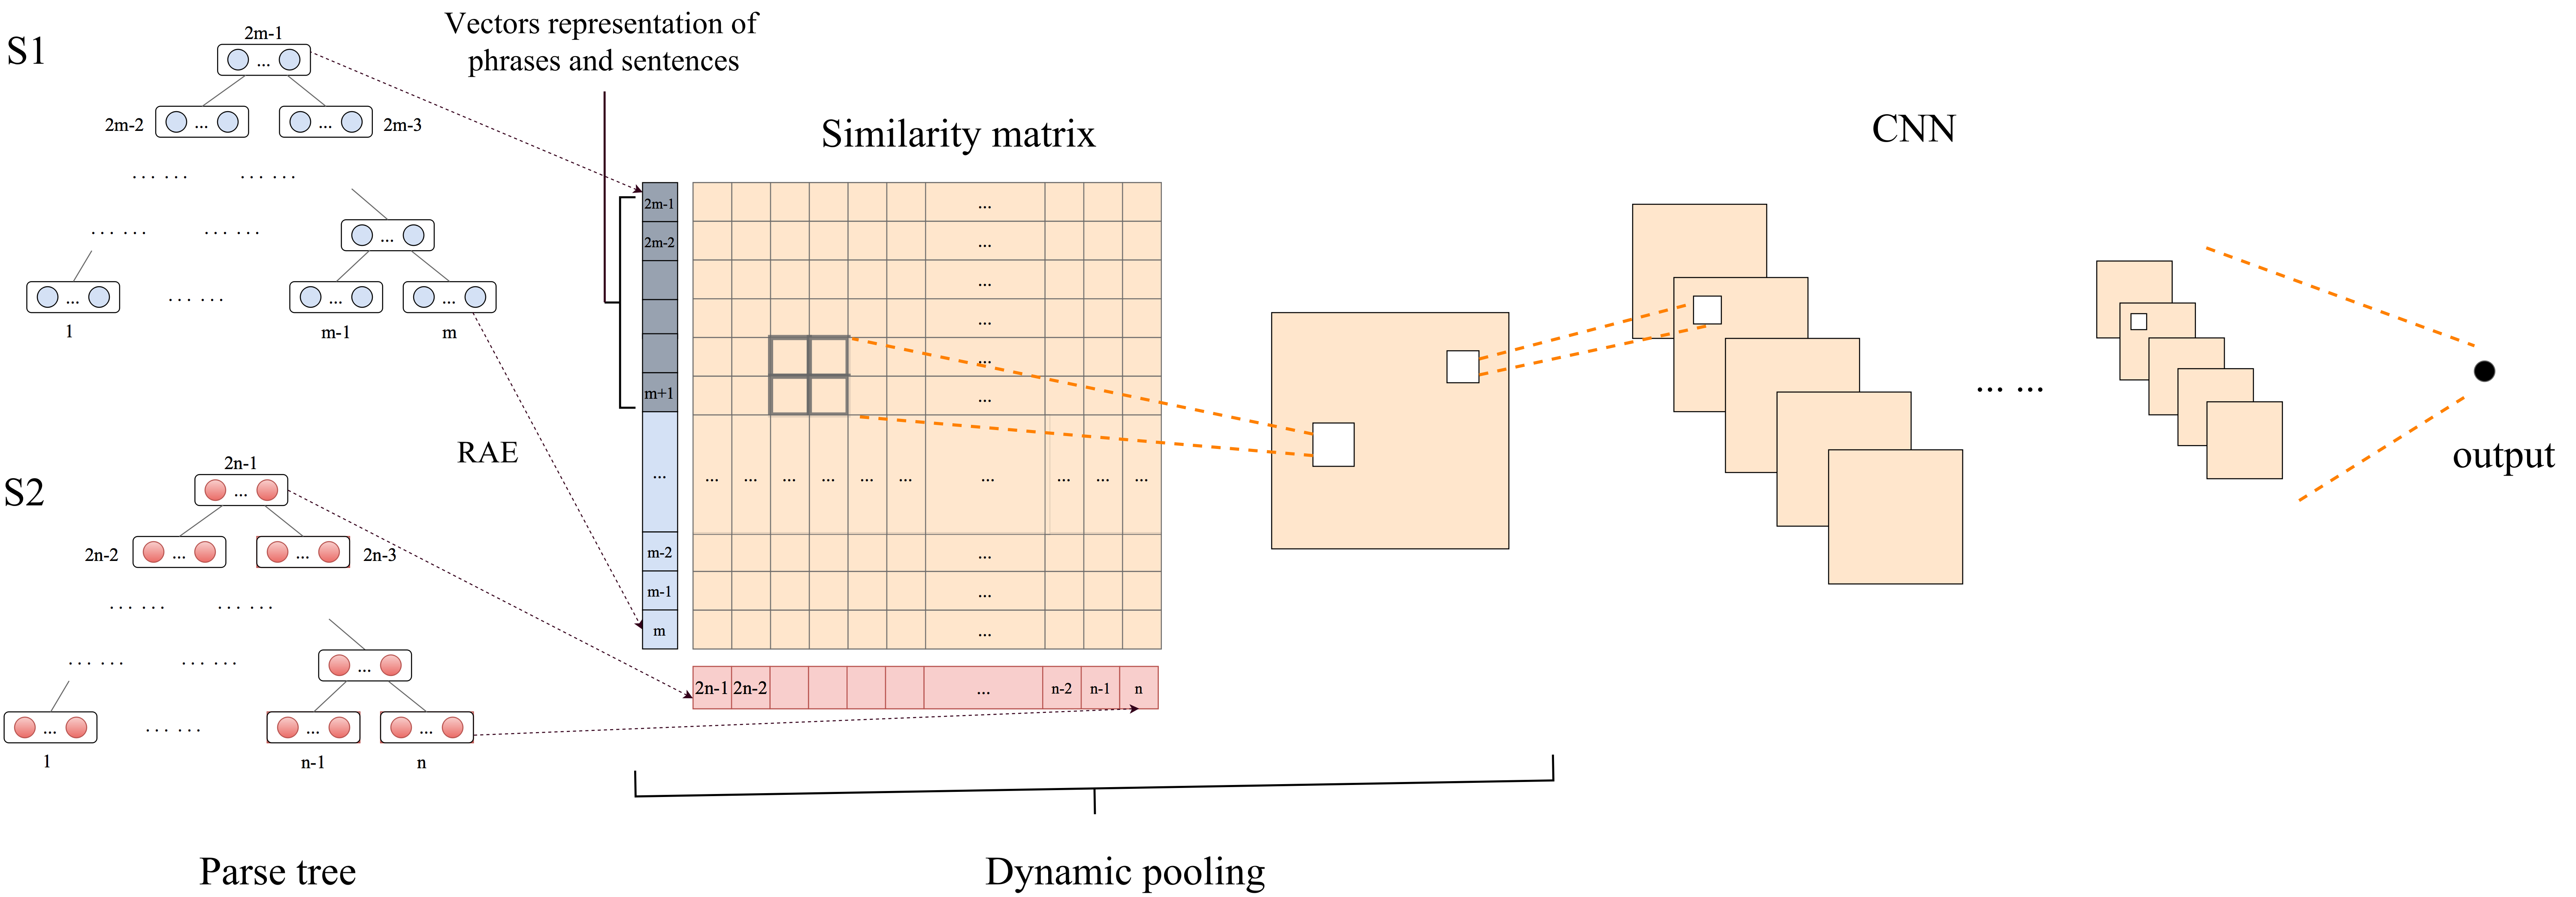
\includegraphics[width=0.9\textwidth]{figures/Overall}
	\caption{The Overall Framework}
	\label{fig:overall}
\end{figure*}

\subsection{Word Representation}

Word embedding nowadays has become the basis of various natural language processing tasks. The purpose of word embedding is to represent word in a vector space. One of the most classical model is a language model which can learn the representation of word into a low-dimensional space and predict a word when given its context \cite{DBLP:conf/icml/MnihT12}. As such semantic information of word can be represented by such a low-dimensional word embedding. In this research, we just follow the work presented in \cite{DBLP:conf/nips/SocherHPNM11} and adopt the 100-dimentional vectors trained by the unsupervised method in \cite{DBLP:conf/icml/CollobertW08}. %. [28] obtain the word representation by using statistic way of collecting the co-occurrence of words and [29] used a neural-network based architecture to train these word embeddings.

Once the word embeddings are learned, we can represent a sentence as $(x_1,x_2, \ldots,x_n)$, where $x_i$ is the vector representation of each word. We use them to create similarity matrix and use them as the leaf nodes of a parse tree to obtain the vectors representation of phrases and sentences.

\subsection{Vectors Representation of Phrases and Sentences}
%Figure1: architecture of Unfolding Recuresive Autoencoder based on a parse tree

In this paper, parse tree is also employed to represent the sentences. The leaf nodes of the parse tree is vector representation of words in a given sentence. The purpose of the Unfolding Recursive Autoencoder is get the vectors representation for nodes from that leaf nodes, which represent the phrases and sentence.

We simply introduce the method of RAE proposed by \cite{DBLP:conf/naacl/YinS15}. Given a list of word vectors $x=(x_1,x_2,\ldots,x_n)$, based on the tree structure given by a syntactic parser, an auto-encoder is learned to map sentences into vectors. In the encoding step, the parents node is calculated by a standard neural network layer from its children:
\begin{equation}
y_1=f(W_e [x_2;x_3]+b)
\end{equation}
where $[x_2;x_3]$ is simply the concatenation of the two children, $f$ is an element-wise activation function such as $\mathit{tanh}$ and $W_e \in \mathbb{R}^{n \times 2n}$ the encoding matrix need to learn. In the decoding step, The unfolding produces the reconstructed leaves by starting at $y_2$ and computing.
\begin{equation}
[x’_1;y’_1]=f(W_d y_2 +b)
\end{equation}

The reconstruction error is then computed from a concatenation of the word vectors in that node's span.
\begin{equation}
E_{rec}(y_{(I,j)})=\|[x_i;\cdots; x_j]- [x'_i;\cdots ;x'_j]\|^2
\end{equation}

After learning the vectors of phrases and sentence, the whole sentence is represented as $(x_1,x_2,\cdots,x_n,x_{n+1},\cdots,x_{2n-1})$, where $ x_1,x_2,\cdots,x_n $ are word vectors, and $x_{n+1},x_{n+2},\cdots,x_{2n-2}$ are phrase vetors and $x_{2n-1}$ is sentence vector. This sentence representation is also used to create similarity matrix.

\subsection{Sentences Pairs Representation}
%\subsection{Similarity Matrix}
Consider a pair of sentences $ S1:(x_1^1,x_2^1,\cdots,x_m^1) $ and $ S2:(x_1^2,x_2^2,\cdots,x_m^2 )$ where $m$ and $n$ is the length of sentences respectively. According to S-Matrix in \cite{DBLP:conf/aaai/ShenRSOX15}, we can map this pair of sentences to a similarity matrix $\sum$ of size $n*m$, in which the each item is defined as below:
\begin{equation}
\delta_{ij}=\cos (x_i^1,x_j^2)
\end{equation}

In this research, we will discuss and compare three types of similarity matrix. Each matrix has the same rows and columns.

1. Each sentence is represented as $(x_1,x_2,x_3,\cdots,x_n)$, and $x_i$ are the word embeddings in correspond position of sentence. We use this sentence representations to create a similarity matrix mentioned above. And then the matrix is tiled to a fixed size:
\begin{equation}
\delta_{ij}=\cos (x_{I \mod m}^1,x_{j \mod n}^2)
\end{equation}

2. Each sentence is represented as $(x_1,x_2,\cdots,x_n,x_{n+1},\cdots,x_{2n-1})$, besides word embedding like (1), $(x_{n+1},\cdots,x_{2n-1})$ are phrases and sentence representation trained from unfolding Recursive Autoencoder of [10]. And then the matrix is tiled to a fixed size.

3. After obtaining the S-matrix mention in (2) before tile, we use the way of dynamic pooling to map the matrix into a fixed size rather than tile.

These similarity matrix are then used as the input of the next CNN architecture.

\subsection{Prediction}

Restricted by the size of the datasets, unlikely the quantity of parameters mentioned in \cite{DBLP:conf/aaai/ShenRSOX15}, we have to carefully control the number of parameters trained in CNN. As such we did are: (1) canceling the final fully connected layer; (2) adding another convolutional layer; and (3) using dynamic filter size, as shown in Fig. \ref{fig:cnn}.

\begin{figure}
	\centering
	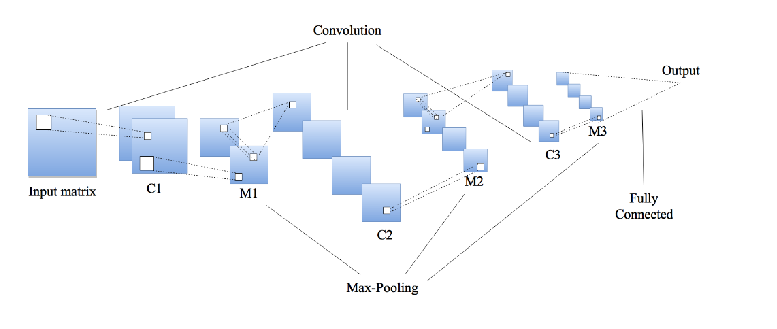
\includegraphics[width=0.9\columnwidth]{figures/Framework}
	\caption{Architecture of Deep Convolutional Neural Network. C1, C2, C3 are convolutional layers with 5 feature maps. M1, M2 ,M3 are max-pooling layer. Each unit in max-pooling layer is connected to a 2×2 neighborhood in the previous convolutional layer. The Output is fully connected with the last pooling layer M3}
	\label{fig:cnn}
\end{figure}

In term of that we have different size of input matrix, and in the experiment, we find that if we apply the same size filter to those input matrix all the time, the performance would be quite worse. If the filter size is too large, it is easy to overfitting. If the input size if too large and the filter size is too small, the model is hard to learn. So we propose a method to choose the filter size $filter(s_f)$ dynamically based on the size of input $matrix(s_i)$.
\begin{equation}
s_m = \lfloor s_i - s_f +1 \rfloor / s_p
\end{equation}
where $s_m$ is the size of feature map after pooling, $s_p$ is the size of pooling matrix. Our method is try to fix the size of the last feature map but ensure the size of filter not to be two large. Our CNN architecture has the following three layers.
\begin{eqnarray}
s_m = \lfloor \frac{\lfloor \frac{\lfloor s_i - s_f + 1\rfloor}{s_p} - s_f + 1\rfloor}{s_p} - s_f + 1 \rfloor / s_p
\end{eqnarray}

In this research, we fixed the size of last layer feature maps to $2 \times 2$, and the size of pooling matrix is $2 \times 2$. And in order to control the number of parameters, we set the size of filer is not larger than 6. So the relationship between size of $filter(s_f)$ and size of input $matrix(s_i)$ is:
\begin{equation}
s_f= \min (\lfloor \frac{s_i -14}{7} \rfloor,6)
\end{equation}

Furthermore, following the suggestion in \cite{DBLP:conf/nips/SocherHPNM11}, we also incorporate some number features. We combine the last output of the layer of CNN and these number features and map to hidden layer as shown in Fig. \ref{fig:rae}.

\begin{figure}
	\centering
	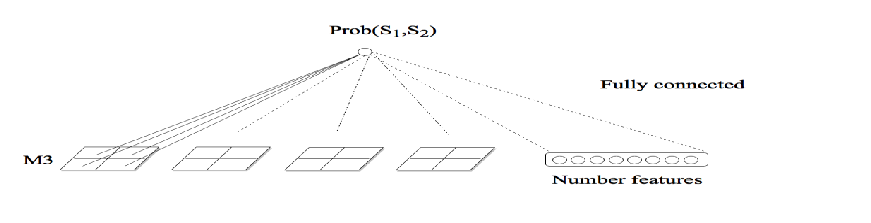
\includegraphics[width=0.9\columnwidth]{figures/Predication}
	\caption{Prediction combining the number features}
	\label{fig:rae}
\end{figure}


\section{Experimental Study}
\subsection{Dataset}
In this section, we demonstrate our proposed method on Microsoft Research Paraphrase Corpus (MSRPC), which is a commonly used dataset for paraphrase identification. It consists of 5,801 sentence pairs. We used the standard split of 4,076 training pairs (67.5\% of which are paraphrases) and 1,725 test pairs (66.5\% of which are paraphrases). The average of length of the sentences is 21, the shortest sentence has 7 words, and the longest one has 36 words. The evaluation metrics will use the traditional Accuracy and F1.

\subsection{Hyperparameters and Training Details}
we chose the negative log-likelihood as out cost function, which is also called cross-entropy cost function. The paraphrase identification task is a binary classification problem. So the cost function $J(\theta)$ can be written as:
\begin{equation}
J(\theta) = -\sum_{i} (t_i \log y_i + (1-t_i)(1- \log y_i))
\end{equation}
where $t_i$ is the target, and $y_i$ is our model’s prediction which is the probability of the two sentences are paraphrased. We further add L2-regularization after the cost function.
\begin{equation}
J(\theta) = -\sum_{i} (t_i \log y_i + (1-t_i)(1- \log y_i)) + \beta || \theta ||^2
\end{equation}

%And we used mini-batch gradient descent optimization method described as follow:
For training process, in this research we adopted a minibatch size of 50, a learning rate of 0.04, and a per-minibatch L2 regularization strength of $10^{-4}$. We also employed the 100-dimentional vectors trained by the unsupervised method \cite{DBLP:conf/icml/CollobertW08}, while the word vectors do not updated in our model. As to the CNN model, each convolutional layer in our proposed model has 5 feature maps. Furthermore, we will compare our proposed model against multilayer perception (MLP) based method in the following section. With regard the setting for MLP, we adopted two layers MLP model and the each hidden layer has 100 neurons.

\subsection{Evaluation Metrics}
F-measure and accuracy are the official evaluation metrics used to rank this task. Assume that the original samples are separated into two categories: positive samples and negative samples. The output of prediction can be classified as true positive ($tp)$), true negative ($tn$), false positive ($fp$), and false negative ($fp$). As such the evaluation metrics can be defined as:
\begin{equation}
Precision = \frac{tp}{tp + fp}
\end{equation}
\begin{equation}
Recall = \frac{tp}{tp + fn}
\end{equation}
\begin{equation}
Accuracy = \frac{tp+tn}{tp + tn + fp + fn}
\end{equation}
\begin{equation}
F1 = 2\frac{Precsion \times Recall}{Precision + Recall}
\end{equation}


\subsection{Results and Discussion}
The first experimental study will test the difference of the three types of representation of the relationship between sentences as mentioned in section 3, i.e., (a) Word embedding + Tile; (b) Word embedding + RAE + tile; (c) Word embedding + RAE + dynamic pooling. We used the parameters of RAE trained in \cite{DBLP:conf/nips/SocherHPNM11} to create the matrix of (b) and (c).

\begin{figure}
	\centering
	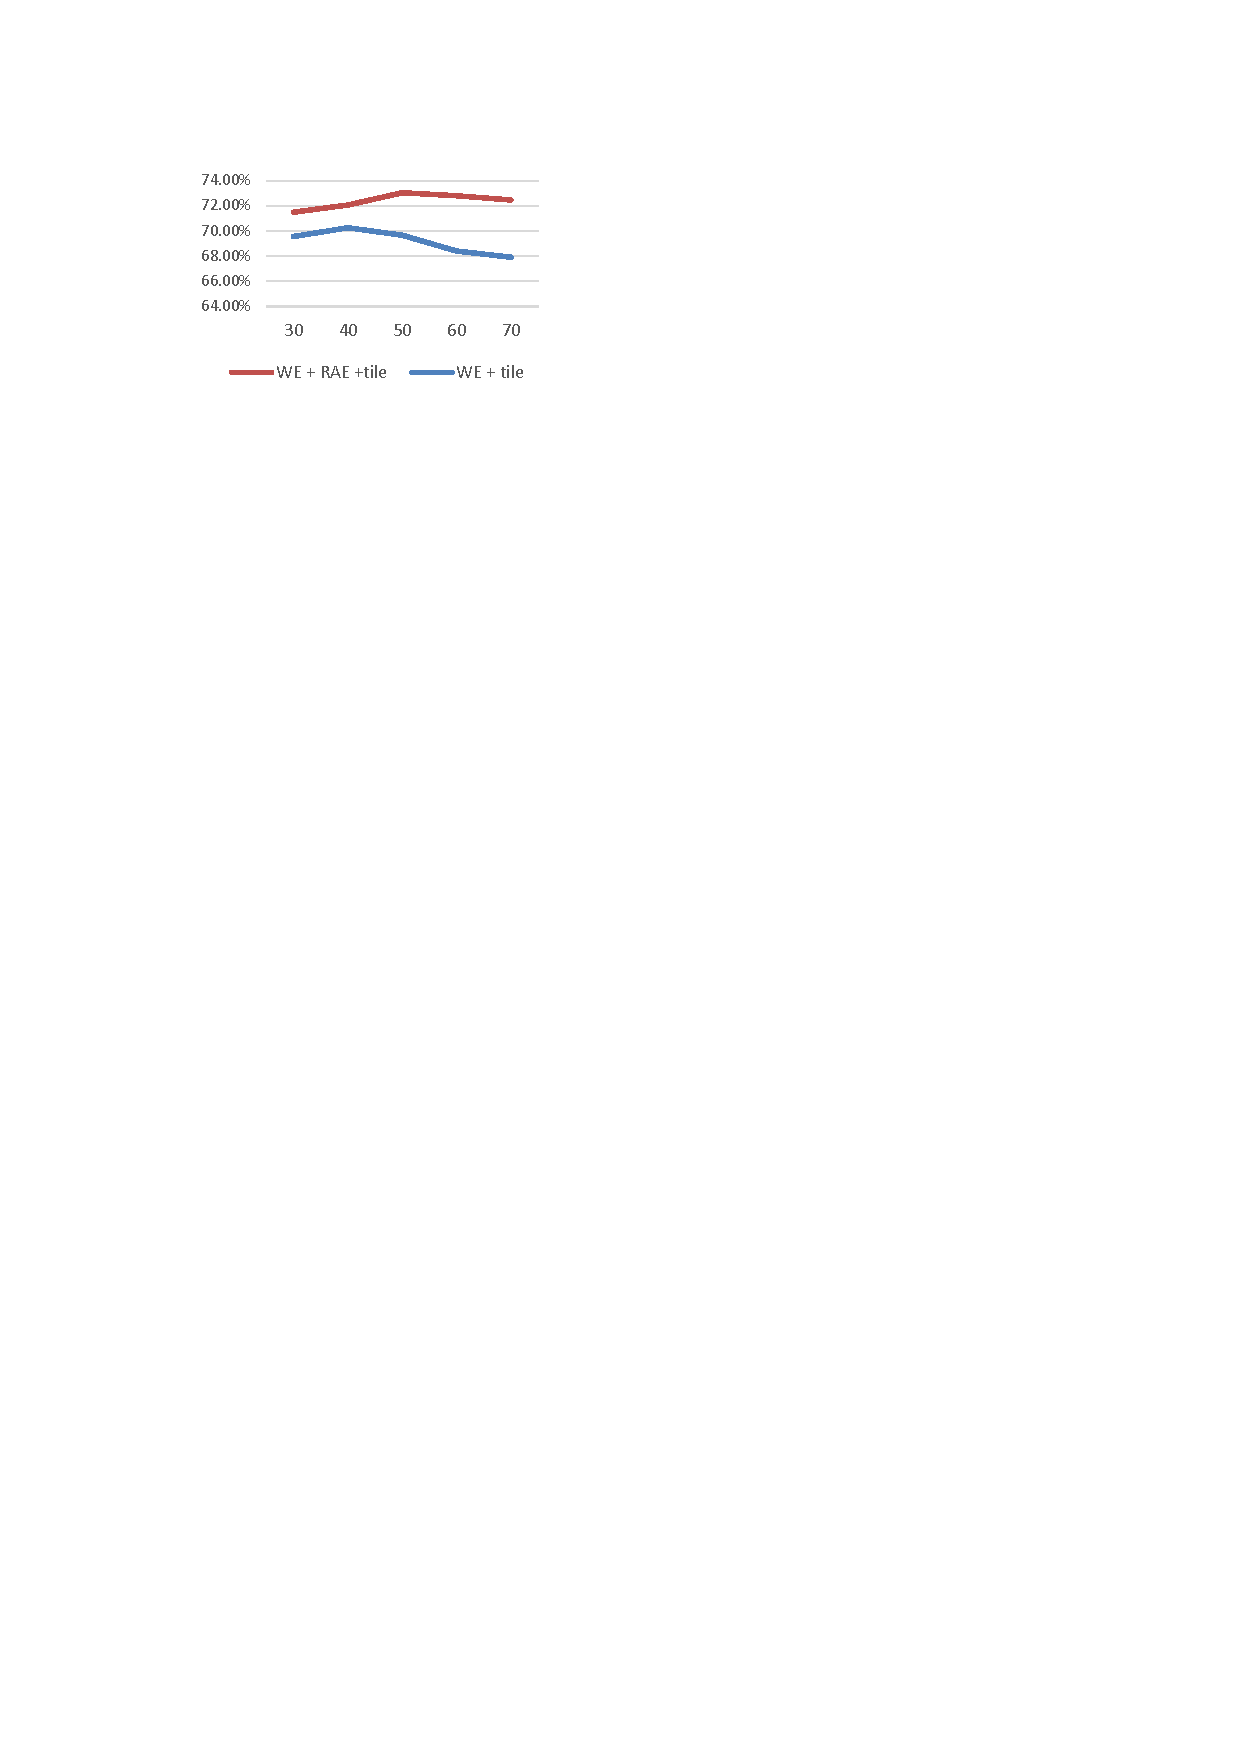
\includegraphics[width=0.9\columnwidth]{figures/Evolution.pdf}
	\caption{Evolution of accuracy with different size of matrix after tile}
	\label{fig:evolution}
\end{figure}

In order to evaluate whether a pair of sentences are paraphrased or not, we used these matrix as input to Logistic Regression (LR), Multi-Layer Perceptron (MLP) and CNN. In order to control the number of parameters, we applied CNN with two convolutional layers to matrix got from (c), and the filter size is $2 \times 2$; we applied CNN with three convolutional layers to matrix obtained from (a) and (b), while the filter size is dynamic. Figure \ref{fig:evolution} shows the evolution of accuracy with different size of matrix after tile. It is observed that 40 x 40 is the best choice for (a), and 50 x 50 is the best choice for (b).

\begin{table*}[!t]
	\center
	\caption{Performance of LR, MLP, and CNN on three different types of Similarity matrix}
	\begin{tabular}{|l|c|c|c|c|c|c|}
		\hline
		\multirow{2}{*}{Input Matrix} & \multicolumn{2}{c|}{Logistic Regression} & \multicolumn{2}{c|}{MLP} & \multicolumn{2}{c|}{CNN} \\
		\cline{2-7}
		& Accuracy & F1      & Accuracy & F1      & Accuracy & F1      \\ \hline
		WE+Title           & 68.29\%  & 81.11\% & 69.10\%  & 80.38\% & 70.26\%  & 79.97\% \\ \hline
		WE + RAE + tile    & 70.03\%  & 81.44\% & 70.03\%  & 81.44\% & 73.04\%  & 82.18\% \\ \hline
		WE + RAE + pooling & 71.48\%  & 82.27\%	& 72.17\%  & 82.36\% & 73.33\%  & 82.50\% \\ \hline
	\end{tabular}
	\label{tb1}
\end{table*}

\begin{table*}[!t]
	\center
	\caption{Performance on three different types of Similarity matrix with number features (NF)}
	\begin{tabular}{|l|c|c|c|c|c|c|}
		\hline
		\multirow{2}{*}{Input Matrix} & \multicolumn{2}{c|}{Logistic Regression} & \multicolumn{2}{c|}{MLP}& \multicolumn{2}{c|}{CNN} \\
		\cline{2-7}
		& Accuracy & F1      & Accuracy & F1      & Accuracy & F1      \\ \hline
		WE + title + NF         & 74.32\%  & 82.44\% & 74.55\%  & 82.12\% & 75.01\%  & 82.75\% \\ \hline
		WE + RAE + tile +NF     & 74.49\%  & 83.06\% & 74.49\%  & 83.06\% & 77.10\%  & 83.97\% \\ \hline
		WE + RAE + pooling + NF & 76.41\%  & 83.30\% & 76.93\%  & 83.75\% & 77.51\%  & 84.38\% \\ \hline
	\end{tabular}
	\label{tb1}
\end{table*}

\begin{table}[!t]
	\center
	\caption{Test results on MSRP datasets}
	\begin{tabular}{|l|c|c|} \hline
		Model                          & Accuracy   & F1      \\ \hline
		Mihalcea et al. (2006)         & 65.40\%	& 75.30\% \\ \hline
		Kozareva and Montoyo (2006)	   & 76.60\%	& 79.60\% \\ \hline
		Hassan (2011)	               & 68.80\%	& 79.90\% \\ \hline
		Hu et al. (2014) ARC-I	       & 69.60\% 	& 80.30\%  \\ \hline
		Hu et al. (2014) ARC-II	       & 69.90\% 	& 80.90\%  \\ \hline
		Rus et al. (2008)	           & 70.60\%	& 80.50\% \\ \hline
		Mihalcea et al. (2006)	       & 70.30\%	& 81.30\% \\ \hline
		Islam and Inkpen (2007)	       & 72.60\%	& 81.30\% \\ \hline
		Yin et al. (2015)(without pretraining)	& 72.50\% &	81.40\% \\ \hline
		Zia and Wasif (2012)	       & 74.70\%	& 81.80\% \\ \hline
		Fernando and Stevenson (2008)  & 74.10\%	& 82.40\% \\ \hline
		Wan et al. (2006)	           & 75.60\%	& 83.00\% \\ \hline
        Pang et al.(2016)              & 75.94\%    & 83.01\% \\ \hline
		Socher et al. (2011)	       & 76.80\%	& 83.60\% \\ \hline
		Madnani et al. (2012)	       & 77.40\%	    & 84.10\%  \\ \hline
		Yin et al. (2015)(with pretraining)	& 78.10\% &	84.40\% \\ \hline
		%		Ji and Eisenstein (2013)	   & 80.4\%	    & 85.9\% \\ \hline
		WE + RAE + CNN	               & 77.51\%	& 84.38\% \\ \hline
	\end{tabular}
	\label{tb1}
\end{table}

The detailed experimental result is shown in Tables 1-3. From Table 1, it is found that the result of matrix created by RAE is always better than matrix not by RAE, and nearly all the results of neural network models by MLP and CNN are always better than the Logistic Regression, which indicates the advantages of deep neural network and the representation of sentences with more information, except for the result of MLP combined the input matrix made by method(b), which might be caused by too many parameters. Besides, we can also see that the results of CNN are always better than the results of MLP, which means that the CNN model is able to discover deeper relationship of two sentences. From table 2, we can also see the same trends when combining the number features. Furthermore, the dynamic pooling seems to be a better way than tile to deal with the problem of fixed size.

Finally, We compared our results against several methods: cosine similarity with tf-idf weighting \cite{DBLP:conf/aaai/MihalceaCS06}; explicit semantic space by \cite{hassan2011measuring}; combination of lexical and semantic features by \cite{DBLP:conf/fintal/KozarevaM06}; graph subsumption \cite{DBLP:conf/flairs/RusMLMG08}; combination of several word similarity measures \cite{DBLP:conf/aaai/MihalceaCS06}; combination of semantic and string similarity \cite{islam2009semantic}; semantic heuristic features by \cite{ul2012paraphrase}; JCN WordNet similarity with matrix by \cite{fernando2008semantic}; dependency-based features \cite{selfdef:conf/altw/WanDDP06}; recursive autoencoder with dynamic pooling by \cite{DBLP:conf/nips/SocherHPNM11}; combination of eight machine translation metrics by \cite{DBLP:conf/naacl/MadnaniTC12}; CNN model without/with pretraining technique \cite{DBLP:conf/naacl/YinS15}; Convolutional neural network architectures for matching natural language sentences by \cite{DBLP:conf/nips/HuLLC14, DBLP:conf/aaai/PangLGXWC16}.

Table 3 shows that our method achieve better performance than most of those state-of-the-art methods. Our method is also superior to recent neural network model \cite{DBLP:conf/nips/HuLLC14, DBLP:conf/aaai/PangLGXWC16}. There is an interesting point with regard to the method proposed in \cite{DBLP:conf/naacl/YinS15}, the proposed model can only overcome its version without pretaining but only present competitive performance against its version with pretraining. Though with pretraining can enhance the overall performance, it is believed that it will cost extra resources for the training process. But it did give our method some room to further improve.

%\cite{DBLP:conf/emnlp/JiE13} used unsupervised learning method and rich sparse features, obtaining the best result on MSRP.

%PI using semantic heuristic features by [20];

\section{Conclusion and Future Work}
Paraphrase identification is a fundamental task in the area of natural language process. Some work use statistical classifier based on exploring the lexical features on both word and character levels, while other approaches tried to model the syntactic-based features on parse structures of two sentences. With the development of deep learning technology, some scholars employed CNN to conduct natural language process tasks. Inspired by the previous work, it is interesting to ask if those information can be integrated together. In this research, it is found that a better representation of relation between two sentences, containing syntactic and semantic information could be helpful when employing deep neural network like CNN. In future work, we might use the vectors, which could represent the word and its context rather than only word to create similarity matrix \cite{DBLP:conf/conll/MelamudGD16}. Such a similarity matrix might also be promising.

\section*{Acknowledgements}
This work was partially supported by the National Natural Science Foundation of China (No. 61472021), the National Department Public Benefit Research Foundation (No. 201510209), and the Fundamental Research Funds for the Central Universities.
%This work was partially supported by the xxx.


% trigger a \newpage just before the given reference
% number - used to balance the columns on the last page
% adjust value as needed - may need to be readjusted if
% the document is modified later
%\IEEEtriggeratref{8}
% The "triggered" command can be changed if desired:
%\IEEEtriggercmd{\enlargethispage{-5in}}

% references section

% can use a bibliography generated by BibTeX as a .bbl file
% BibTeX documentation can be easily obtained at:
% http://www.ctan.org/tex-archive/biblio/bibtex/contrib/doc/
% The IEEEtran BibTeX style support page is at:
% http://www.michaelshell.org/tex/ieeetran/bibtex/
%\bibliographystyle{IEEEtran}
% argument is your BibTeX string definitions and bibliography database(s)
%\bibliography{IEEEabrv,../bib/paper}
%
% <OR> manually copy in the resultant .bbl file
% set second argument of \begin to the number of references
% (used to reserve space for the reference number labels box)
% control reference type settings
\IEEEtriggeratref{19}
\bibliographystyle{IEEEtran}
\bibliography{reference}

% that's all folks
\end{document}


